\chapter{State Transformers: Models and Automation}
\label{chap:transformers}

This chapter discusses \JV's state transformation model in more detail. We
present \JV's per-type object transformation model; our use of state
transformers to repair application state for specific bugfixes; and a
methodology
for automating state transformer generation to ease programmer burden.


\section{Object Transformation Model}
\label{sec:transformer-model}

% \todo{Fix this}
% This section explains \JV's object transformation model and discusses its
% limitations and alternatives. We first go over an example of a simple
% update, how intuitive transformers express this update, and how they lead to
% our chosen model. We then revisit our singly-linked to doubly-linked
% example introduced in Section~\ref{sec:xformers}.

This section explains \JV's object transformation model and compares it to
other alternatives by revisiting the singly-linked to doubly-linked example
introduced in Section~\ref{sec:xformers}.

% \JV provides to the
% user and our rationale. We go over the simple change in
% Figure~\ref{fig:two-classes-change} and argue that developers will find
% this model intuitive.

Any dynamic updating system must convert old process state at
the time of the update to the one expected by the new version at the point it
resumes execution. The system must convert state maintained in global
static data, method stack variables, and heap data as required for the new
version. Even ignoring semantics of the application, at the very least, the
system needs to represent data correctly in the form expected by the new
version.

In an object-oriented programming language like Java, data is primarily
stored as objects in the heap. An object is statically-typed\footnote{In
contrast, dynamically-typed languages such as Python may change fields
and methods of an object over time, and objects of the same class
need not be consistent.}, and is an instance of a particular {\tt class}.
A dynamic updating system for Java should convert heap objects to the new version in a
class-specific manner, leading to class or type-specific
object transformation functions \cite{neamtiu06dsu, K42reconfig}.
% In \JV's case, are \JO functions.
Such a type-specific transformation function specifies how to obtain an
object of the new version's type given an object of the old one. As
explained in Section~\ref{sec:updating-data}, there exist two main design
choices on when to execute these transformation functions. One design is to
lazily transform objects. In a lazy approach, objects are transformed when
they are first accessed by the application after the update. A lazy
approach requires that application code be instrumented to check the state
of an object and transform it if necessary. The other design alternative is
to eagerly identify and transform all objects at once. For \JV, we followed
the eager approach because we did not want to incur the steady-state
performance overhead that comes with instrumenting code and because we
could efficiently transform the entire heap by piggybacking on garbage collection. We
first discuss design choices with the eager transformation model and then
present the lazy transformation model and how one might implement it in
\JV.

\subsection{Eager transformation models}

For the rest of this discussion, we assume that the interface to specify
object transformers is the \JO function. This function accepts two
parameters: an object corresponding to the old version called \FROM and an
object for the new version called \TO. The programmer specifies how to
initialize the \TO object with data from the \FROM object.  The
interesting question in this and other models is,
what the types of the \FROM and \TO parameters
should be. We require access to the both the old and new version's
definition, yet we must not break Java's type system in order to utilize
the strong type-safety guarantees provided by the language. The definitions
of the \FROM and \TO objects depend on what view of the heap
the developer uses during transformation time and vice versa. In one, the
programmer has access to the old version's code and any pointer dereference
will return an object that is consistent with the old version.  We call
this model the ``old world'' model. In the ``new world'' model, the programmer has access to
the new version's code and any pointer dereference will return an object of
the new version. The old world model
has some natural advantages over the new world model. Since the old world
model presents the well-formed old heap from before the update, any code or
data access on this heap will be safe. The new world model exposes the
transformation function to a heap that is yet to be populated.  Dereferencing
pointers to objects whose contents are yet filled can result in
incorrect data values or null pointer exceptions. Before transformer
code can access an object, the programmer or the compiler has to ensure
that its contents are correctly filled in. In \JV we implemented the new
world model because it integrated naturally with our VM implementation.

\begin{figure}[t]
\lstset{frame=single}
\begin{tabular}{@{}m{0.5\textwidth}@{}m{0.5\textwidth}@{}}
\BC \begin{minipage}{0.3\textwidth}
\begin{lstlisting}
public class X {
  private Y y;
}
public class Y {
  private int i;
}
\end{lstlisting}
\end{minipage} \EC &
\BC \begin{minipage}{0.32\textwidth}
\begin{lstlisting}
public class X {
  private String s;
  private Y y;
}
public class Y {
  private int i, j;
}
\end{lstlisting}
\end{minipage} \EC \\[-3ex]
\BC (a) Old version \EC &
\BC (b) New version \EC \\[-2ex]
\end{tabular}
\hangcaption{Example of a simple update where the field of an updated class
refers to another updated class\label{fig:two-classes-change-only-diff}}
\lstset{frame=none}
\VspaceFixForHangcaption
\end{figure}

% \begin{figure}[t]
\lstset{frame=single}
\begin{tabular}{@{}m{0.5\textwidth}@{}m{0.5\textwidth}@{}}
\BC \begin{minipage}{0.3\textwidth}
\begin{lstlisting}
public class X {
  private Y y;
}
public class Y {
  private int i;
}
\end{lstlisting}
\end{minipage} \EC &
\BC \begin{minipage}{0.32\textwidth}
\begin{lstlisting}
public class X {
  String s;
  private Y y;
}
public class Y {
  private int i, j;
}
\end{lstlisting}
\end{minipage} \EC \\[-3ex]
\BC (a) Old version \EC &
\BC (b) New version \EC \\[-2ex]
\end{tabular}
\BC \begin{minipage}{0.75\textwidth}
\begin{lstlisting}
class old_X { public Y y; }
class old_Y { public int i; }
class JvolveTransformers {
  public static void
      jvolveObject(X to, old_X from) {
    to.s = null; to.y = from.y;
  }
  public static void
      jvolveObject(Y to, old_Y from) {
    to.i = from.i; to.j = 0;
  }
}
\end{lstlisting}
\vspace{-1ex} \BC (c) Stub classes used in transformers \EC
\end{minipage} \EC
\hangcaption{Example of a simple update where the field of an updated class
refers to another updated class\label{fig:two-classes-change}}
\VspaceFixForHangcaption
\lstset{frame=none}
\end{figure}


Figure~\ref{fig:two-classes-change-only-diff} shows an example of an update
with two classes {\tt X} and {\tt Y}.  Class {\tt X} has a field {\tt y}
pointing to an object of type {\tt Y}.  The update adds an additional field
each to classes {\tt X} and {\tt Y}.
Figure~\ref{fig:two-classes-change-transformers} shows the object
transformers for classes {\tt X} and {\tt Y} in the old and new world
models. In the old world model, the \FROM parameters are of the old types
{\tt X} and {\tt Y}. The types of the \TO parameters are artificially
constructed stub classes that correspond to the definition of the new
versions of {\tt X} and {\tt Y}. Note that fields of the \nX and \nY
classes, specifically, {\tt \nX.y} refers to an old version object, thus
maintaining the old world invariant. Conversely, in the new world model the \TO
parameters are of the new version's types while the \FROM parameters are
stub classes that correspond to the definition of the old version. The
field {\tt \oX.y} refers to a new version object.

\begin{figure}[p]
\BC
\begin{minipage}{0.62\textwidth}
\begin{lstlisting}[frame=single]
// new_X.y refers to the old version
// The new X and Y do not exist, yet
class new_X { String s; Y y; }
class new_Y { int i, j; }

class JvolveTransformers {
  public static void
      jvolveObject(new_X to, X from) {
    to.s = null; to.y = from.y;
  }
  public static void
      jvolveObject(new_Y to, Y from) {
    to.i = from.i; to.j = 0;
  }
}
\end{lstlisting}
\end{minipage} \\
(a) Old World Model: Stub classes and transformers \\[2ex]
\begin{minipage}{0.62\textwidth}
\begin{lstlisting}[frame=single]
// old_X.Y refers to the new version
// The old X and Y do not exist now
class old_X { public Y y; }
class old_Y { public int i; }

class JvolveTransformers {
  public static void
      jvolveObject(X to, old_X from) {
    to.s = null; to.y = from.y;
  }
  public static void
      jvolveObject(Y to, old_Y from) {
    to.i = from.i; to.j = 0;
  }
}
\end{lstlisting}
\end{minipage} \\
(b) New World Model: Stub classes and transformers \\[2ex]
\hangcaption{Stub classes and transformers for the update in
Figure~\ref{fig:two-classes-change-only-diff}\label{fig:two-classes-change-transformers}}
\EC
\VspaceFixForHangcaption
\end{figure}


In the new world model, the stub classes
\oX and \oY have the same fields (both
types and names) as defined in the old version and provide access to the
fields of old-version objects in a type-safe manner. These stub classes are
used by the Java-to-bytecode compiler to compile object transformer
functions. However, as explained in Section~\ref{sec:loading}, \JV
does not load these classes. It merely renames the old version of the class
that is already loaded by the application to the names of these stubs. This
renaming eliminates the naming conflict between old and new class names. In
the old world model, the runtime replaces stub classes \nX and \nY used while transforming
objects with the new versions of {\tt X} and {\tt Y} before the
application resumes execution.

% Now that we have established sensible type declarations for the \FROM and
% \TO parameters, let us delve a little bit deeper into what the definition
% of \oX and \oY should actually be. The \oY's definition is straightforward.
% It has a single integer field as shown in
% Figure~\ref{fig:two-classes-change}~(c). \oX's definition is a bit more
% involved. The question is whether field {\tt y} should be of type {\tt Y},
% or should it be of type \oY? Do we want it to refer to refer to an object
% of the old version or the object of the new version? Both solutions seem
% reasonable.



% As described in Chapter~\ref{chap:related}, Boyapati et
% al.~\cite{boyapati03lazy} have references to old-version objects. In such a
% system, the programmer has access to the old version's state
% 
% while and
% others~\cite{k42usenix,neamtiu06dsu,neamtiu09stump,upstare} refer to new
% objects. In \JV, we chose the latter approach for the following reason.

\begin{figure}[t]
\begin{center}
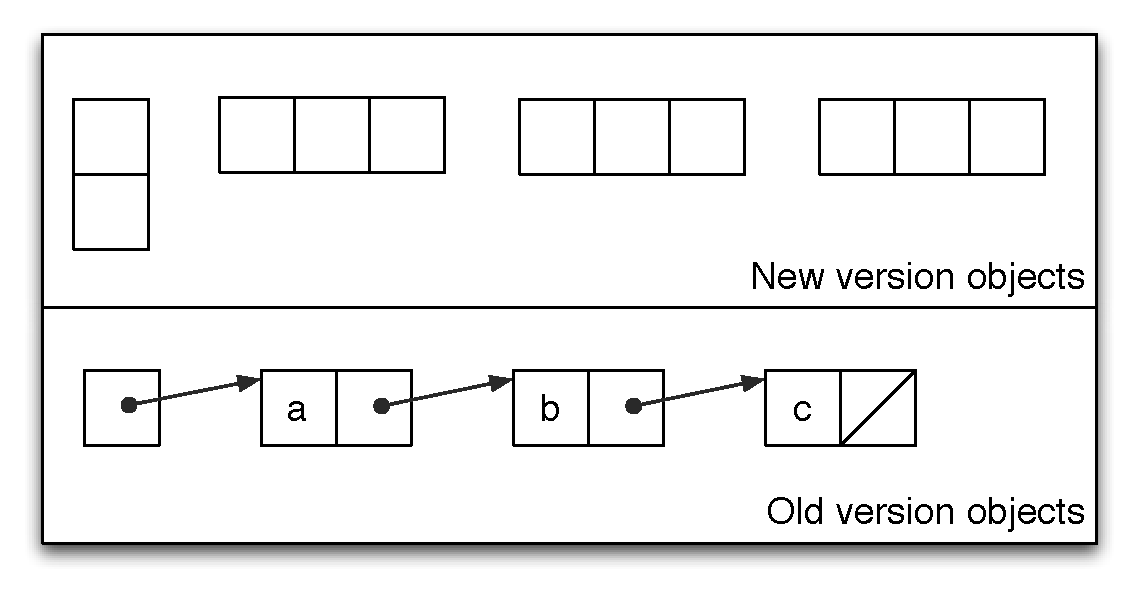
\includegraphics[scale=0.48]{100-images/singly-doubly/old-world-singly-doubly-before-transform}
\\
(a) View of the heap before running object transformers \\[1ex]
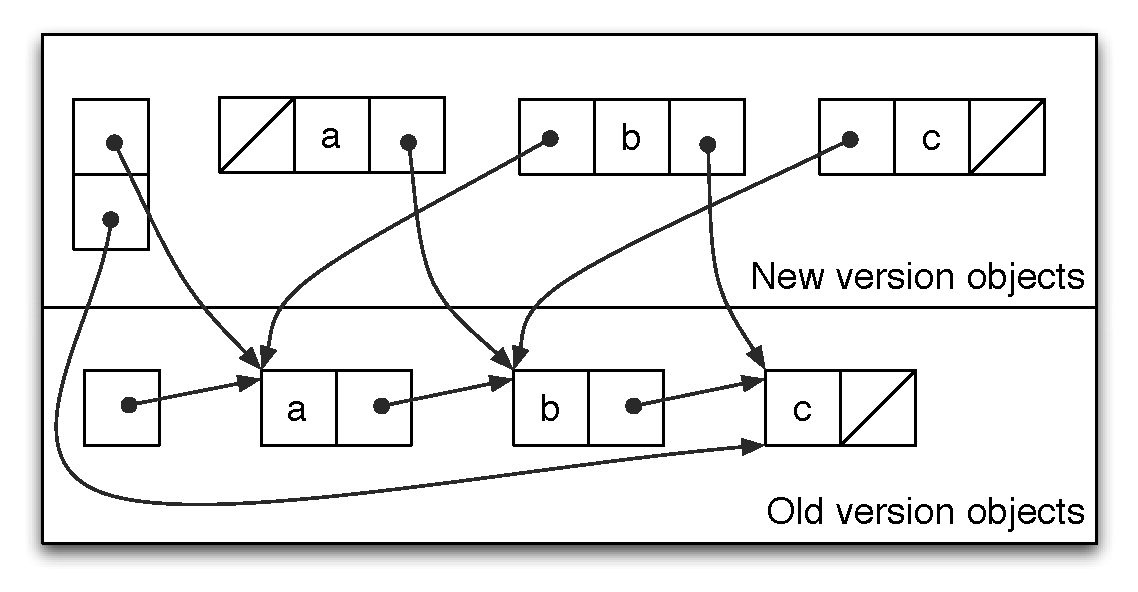
\includegraphics[scale=0.48]{100-images/singly-doubly/old-world-singly-doubly-transformed}
\\
(b) View of the heap after running object transformers \\
\hangcaption{Old World Model: A view of the linked lists, before and
after running transformation functions\label{fig:old-world-heap}}
\VspaceFixForHangcaption
\end{center}
\end{figure}


The simplest meaningful transformer functions possible are those that copy
fields from the old-version object to the new one. In both models, the
programmer can copy both primitive and reference fields. In the old world view,
reference fields point to old version objects, while in the new world view
they point to new version objects. In the old world view, the dynamic
updating system changes every reference to an old version object to its
corresponding new one, before the application resumes execution.

% With \JV we wanted
% to allow the programmer to effortlessly copy fields with a simple
% assignment such as {\tt to.y = from.y}. This choice forces {\tt \oX.y} to be of
% the same type as {\tt X.y} which in this case happens to be the new
% version's {\tt Y}. If {\tt \oX.y} were pointing to an old-version object,
% the programmer would have to explicitly call a special \VM function that would
% pretend that the types were compatible and force the assignment. The
% system would also have to point to new-version objects as required by the
% new version, before resuming execution.  This conflict motivates our choice
% that the types of these
% fields should be of the new-version, we now consider the
% nature of objects referred to by these fields.  Since these are new-version
% objects and types, the question arises as to whether these objects have
% their contents filled in or not at the time a transformer runs.

% \JV's implementation does not
% % currently
% guarantee at the time {\tt X}'s transformer is invoked whether the
% field {\tt y} points to an object waiting to be transformed (and is therefore
% empty), or whether it points to an object that is transformed and has its
% contents filled in. Enforcing an ordering can get tricky especially in the
% presence of circular references. Moreover, {\tt y}'s state is important
% only if the programmer were to dereference the field. It does not matter if
% the transformer merely copies the field {\tt y}. While not the most elegant
% solution, \JV forces the programmer to specify that {\tt y} be transformed
% on-demand, if the transformer needs to dereference the field.
% 
% In summary, \JV updates program state by allowing \UPT or the programmer
% to specify per type transformation functions. These functions receive as
% parameters an object of the old version's type and an object of the new
% version's type. The fields of the old-version object are of the
% new-version type and point to new-version objects. The objects pointed to
% by these fields may or may not be have been transformed when the
% transformer function for the object containing these fields is invoked. The
% programmer can on-demand force these fields to be transformed.

% \todo{Talk about semantics?} With this model, what are our pitfalls now?
% 1) Transformer code may depends on application semantics.  2) Transformer
% code may depends on where we are, in the application.

% \todo{This might look out of place}

\begin{figure}[t]
\BC
\begin{minipage}{0.8\textwidth}
\begin{lstlisting}[frame=single]
public static void jvolveObject(
            r1_LinkedList to, LinkedList from) {
  to.head = from.head;
  Node prev = null;
  Node current = from.head;
  while (current != null) {
    prev = current;
    current = current.next;
  }
  to.tail = prev;
}
\end{lstlisting}
\end{minipage}
\hangcaption{Old World Model: Object Transformers to convert a
singly-linked list into a doubly-linked list\label{fig:old-world-transformer}}
\EC
\VspaceFixForHangcaption
\end{figure}


\paragraph{Updating from a singly-linked list to a doubly-linked list}

We revisit the singly-linked to doubly-linked example from
Figure~\ref{fig:singly-doubly} to explain transformers in the old world and
new world models.  As mentioned in Section~\ref{sec:xformers}, it is
straightforward to set the {\tt head} pointer of the doubly-linked list.
Setting the {\tt tail} pointer to the last node involves traversing the
linked list. In the old world model, the list is well-formed and the
transformer code obtains the last node with a simple traversal of the list.
The new world model requires special handling since it involves traversing
a list whose nodes are yet to be populated.
% Whereas, in the new world model, special care is required

We first present the old world model. Figure~\ref{fig:old-world-heap} shows
the heap before and after running object transformers. The heap
is logically divided into objects of the old version and those of the new
version. All pointers refer to objects of the old version. The object
transformer functions given in Figure~\ref{fig:old-world-transformer}
populate the empty new version objects. The code to set the {\tt tail}
field of the list involves a simple list traversal. After transforming all
objects the dynamic updating system scans the heap and converts all
pointers to refer to the new version objects and the application can resume
execution. After this phase, the heap is identical to the new world heap
after transformation shown in Figure~\ref{fig:new-world-heap}~(b).

Converting the singly-linked list to a doubly-linked list in the new world
model is a bit more involved. Figure~\ref{fig:new-world-heap} shows a view
of the heap before and after running object transformers in the new world
model. All pointers refer to objects of the new version. The heap is ready
to be used by the application immediately after running the transformers.

\begin{figure}[t]
\begin{center}
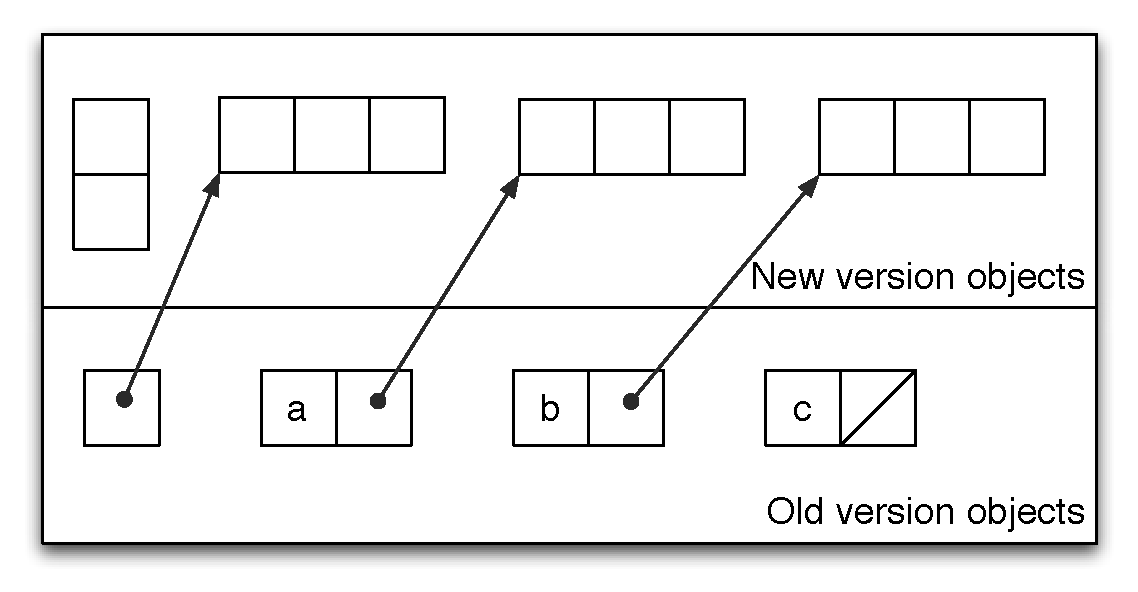
\includegraphics[scale=0.48]{100-images/singly-doubly/new-world-singly-doubly-before-transform}
\\
(a) View of the heap before running object transformers \\[1ex]
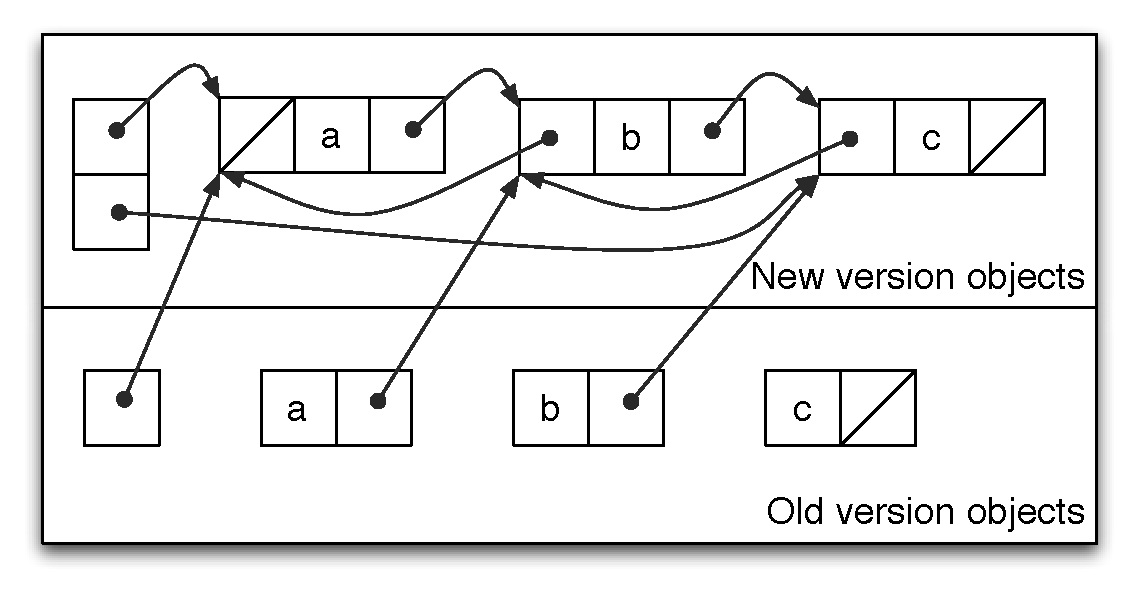
\includegraphics[scale=0.48]{100-images/singly-doubly/new-world-singly-doubly-transformed}
\\
(b) View of the heap after running object transformers \\
\hangcaption{New World Model: A view of the linked lists, before and
after running transformation functions\label{fig:new-world-heap}}
\VspaceFixForHangcaption
\end{center}
\end{figure}

\begin{figure}[p]
\lstset{frame=single}
\BC \begin{tabular}{@{}c@{}}
% \begin{minipage}{0.85\textwidth}
% \begin{lstlisting}[title={(a) Default \UPT-generated transformer}]
% public static void jvolveObject(
%             LinkedList to, r0_LinkedList from) {
%   to.head = from.head;
%   to.tail = null; // no such field in from
% }
% \end{lstlisting}
% \end{minipage} \\
\begin{minipage}{0.9\textwidth}
\begin{lstlisting}[title={(a) Explicitly traversing old and new version objects}]
public static void jvolveObject(
            LinkedList to, r0_LinkedList from) {
  to.head = from.head;
  Node prev = null;
  Node current = from.head;
  while (current != null) {
    prev = current;
    if (! VM.is_transformed(current)) {
      r0_Node current_old = VM.old_version_object(current);
      current = current_old.next;
    } else {
      current = current.next;
    }
  }
  to.tail = prev;
}
\end{lstlisting}
\end{minipage} \\
\begin{minipage}{0.9\textwidth}
\begin{lstlisting}[title={(b) Explicitly transforming new version objects}]
public static void ensure_transformed(Object o) {
  if (! is_transformed(o)) {
    // The jvolveObject method corresponding to the
    // object's type is invoked using reflection.
    jvolveObject(o, old_version_object(o));
  }
}
public static void jvolveObject(
            LinkedList to, r0_LinkedList from) {
  to.head = from.head;
  Node prev = null;
  Node current = from.head;
  while (current != null) {
    prev = current;
    VM.ensure_transformed(current);
    current = current.next;
  }
  to.tail = prev;
}
\end{lstlisting}
\end{minipage}
\end{tabular}
\vspace*{-2.6ex}
\hangcaption{New World Model: Object Transformers to convert a
singly-linked list into a doubly-linked list\label{fig:setting-tail-field}}
\EC
\lstset{frame=none}
\VspaceFixForHangcaption
\end{figure}


In order to set the {\tt tail} of the list to point to the last node, the
transformer code needs to traverse the list to get to the end. At the time
we traverse the list, not all nodes might have been transformed, because we
cannot always control the order in which objects are transformed. There are two
ways to support this update. One is to allow the programmer to access old
version objects from the new world view by making a request to the runtime.
The other is to provide a way for the programmer to request that an object
be transformed on-demand as the programmer traverses the list to retrieve
the {\tt tail} element of the list.
% Section~\ref{sec:discussion} explores this example in more detail and
% presents alternative models to transform objects.


\paragraph{1. Explicitly traversing old and new-version objects.}
We could traverse the list using both objects of the old version and
objects of the new version. It is important to note that, the system we
currently have ensures type-safety. All reference fields, in the old and
new objects, point to objects of the right type. The issue though is that
fields in new objects might be \NULL because these objects have not
been transformed yet.  The \VM could use meta-data in object headers to provide an \API that allows a
programmer to get the old-version object corresponding to a new-version
object and vice versa. % The \VM could use meta-data in object headers to
% provide this facility.
The programmer should carefully traverse the list,
getting the old-version object of a new-version object, and following the
{\tt next} field of the old-version object.
Figure~\ref{fig:setting-tail-field}~(a) shows the object transformer in
this model.

\paragraph{2. Explicitly transforming new-version objects.}
Another approach would be to traverse the linked list, while ensuring that
the nodes are transformed before we dereference them.
Figure~\ref{fig:setting-tail-field}~(b) shows the object transformer in
this model.  The inherent issue we face is that we want to
enforce an order in which objects are transformed. \JV provides an \API
that allows the programmer to transform a particular object on demand. The
programmer could invoke this function {\tt ensure\_transformed} for each
node as they traverse the list. Note that, this VM function calls {\tt
jvolveObject}, the object transformer if an object is not yet transformed.
This mechanism could potentially lead to a cyclic dependency, i.e., transforming an
object might require that the same object already be transformed.
Currently, we do not
address this problem and leave it to the programmer to guarantee
acyclicity.
We could imagine a more sophisticated approach that analyzes
transformation functions and automatically chooses the order in which they
are invoked. Alternatively, we could automatically instrument the
transformer function to make the required \API calls.
% Like the previous solution, this is inelegant and relies on the
% programmer to get the ordering correct.

% \todo{This was there from the paper. How do we integrate this paragraph
% cleanly?} In our example, the \JO function only copies the contents of the
% old \User object's fields.  More generally, our update model allows old
% object fields to be dereferenced in transformer functions so long as the
% fields point to transformed objects.  If some object $o$ is dereferenced
% while running $p$'s transformer method, but $o$ has not yet been
% transformed, we must find $o$ and pass it and its uninitialized new version
% to the \JO method to initialize it.  Since $p$ points to the new version of
% $o$, we could scan the remainder of the update log to find the old version.
% To avoid this cost, we instead cache a pointer to the old version in the
% new version during the collection.  We take care that \JO functions invoked
% recursively in this manner do not loop infinitely, which would constitute
% one or more ill-defined transformer functions. We detect cycles with a
% simple check, and abort the update.  In our current implementation, the
% programmer uses a special VM function to force a field's referenced object
% to be transformed.  We should be able to handle this case automatically,
% through a read barrier or a simple analysis of the \JO bytecode. 

\subsection{Discussion}
%MWH: moved this. Makes more sense in 2.3
% %MWH: leaving this here, but probably it belongs in 2.3 instead...
% In our update model, if a transformer dereferences an object reference
% which also refers to a transformed object, it refers to the new
% version.  Our experience and that of others%
% ~\cite{k42usenix,neamtiu06dsu,neamtiu09stump,upstare}
% indicate that this model expresses many updates well.  Boyapati et
% al.~\cite{boyapati03lazy} also forbid cycles, but in their model,
% transformers only reference old objects. We explain their model in
% more detail in Section~\ref{sec:related}. We leave to future work a
% detailed investigation of the semantics and expressiveness of both models.

While the object transformer functions written for the old world and new
world models indicate that the old world model provides a simpler logical
model for object transformation, we implemented
the new world model for simplicity of implementation and efficiency. The old world model requires
two traversals of the heap --- one pass to identify objects that need to be
transformed, and another pass to scan and convert all pointers that refer
to old version objects to point to new version ones. The old version model
also requires two steps to load classes of the new version. A first step to
load stub classes to run transformers and another step to load the real
classes of the new version after the update. The new world model on the
other head integrates cleanly with our VM implementation. \JV renames old
classes to stub classes and loads new version classes in a single step.
\JV's modified garbage collector walks through the heap, identifies objects
that need to be updated, creates additional copies for such objects while
ensuring that all references point to these new copies. After invoking
object transformers on all updated objects, the application can resume
execution in the new version.

Our implementation of object transformers uses an extra copy of all updated
objects and adds temporary memory pressure.  We  could copy the old
versions to a special block of memory and reclaim it when the collection
completes. We could avoid extra copies altogether by invoking
object transformer functions during collection.  This approach is more
complicated because our transformer model requires recursively invoking the
collector from the transformer if a dereferenced field has not yet been
processed.  We also would need to use a  GC-time read barrier to follow
forwarding pointers before dereferencing an object in order to determine
whether an object has been transformed.

% In addition, to provide access to the fields 
% of changed objects in transformer functions, we can customize the
% collector to completely process the children first using a postorder
% traversal.  This traversal order would guarantee that any object
% reachable from the object transformer function is sure already initialized.
% Other programming 
% interfaces are possible, too.  For example, Boyapati et al.~\cite{boyapati03lazy}
% take advantage of encapsulation information to allow transformer code
% to access the old versions of pointed-to objects.  Our approach allows
% programs to only see the new versions of objects within transformers,
% similar to the \emph{representation consistency} invariant proposed by
% Stoyle et al.~\cite{StoyleHBSN06}.  We will let future experience
% guide our understanding of which programming interfaces are most
% useful.

% These disadvantages have not proved problematic in practice.  Very often the
% default transformer is sufficient, in which case there is no extra copying.
% The custom object transformer functions we have written are similar to the
% one in Figure~\ref{fig:example-xform}.  By and large, they copy fields
% (either base types or pointers) from the old object to the new one.
% Transformers also tend to allocate new objects for changed or added fields,
% and these new objects may, once again, refer to objects directly pointed to
% by the old object.  In the figure, the new {\tt EmailAddress} objects
% point to the {\tt String}s that used to serve as e-mail addresses in the
% old object.

\subsection{Lazy transformation model}
We use a stop-the-world garbage collection-based approach that requires the
application to pause for the duration of a full heap GC in order to perform
the update. An alternative to this model is applying object transformers
lazily~\cite{ritzau00dynamic,Mala00a,boyapati03lazy,neamtiu06dsu,chen:icse07}.
In a lazy model, the system instruments the application to check, at each
dereference, whether an accessed object is up-to-date and invoke its object
transformer if necessary. The main drawback of this approach is that it
adds overhead during steady state execution. However, the lazy approach is
useful in application contexts that cannot tolerate the pause caused by a
full heap GC.

\BCode[t]{0.67}
\begin{lstlisting}[frame=single]
function getfield(object, field):
    value = object.field
    new_value = ensure_transformed(value)
    if (value != new_value):
        setfield(object, field, new_value)
    return new_value

function getstatic(class, field):
    // similar to getfield
    // uses setstatic

function aaload(array, index):
    // similar to getfield
    // uses aastore

function ensure_transformed(o):
    if o.isForwardingPointer():
        return o.ForwardedValue
    else if o.isUpToDate():
        return o
    else:
        new_o = new Object()
        jvolveObject(new_o, o)
        o = (forwarding pointer to new_o)
        return new_o
\end{lstlisting}
\ECode{Lazy object transformation model
implementation\label{fig:read-barrier}}


The lazy approach can be implemented in \JV by performing the following
steps. 1) At update time, invoke object transformers on all stack local
variables. 2) Maintain the invariant that any object accessed by the
application is up-to-date. We can maintain this invariant by adding
read-barrier code to all object dereferences. An object can be dereferenced
in Java only using one of the following three opcodes: {\tt getfield} that
returns a field from an object; {\tt getstatic} that returns the value of a
global variable; and {\tt aaload} that return an array element. The
read-barrier code to check whether or not an object is transformed can use
the same forwarding pointer mechanism used by the garbage collector while
scanning the heap.  Figure~\ref{fig:read-barrier} shows the code that
implements this functionality.  The first time an object is accessed after
the update, it will be transformed leaving a forwarding pointer in its
place. Future accesses to the object that go through the forwarding pointer
return the transformed object and update the corresponding reference. The
forwarding pointer will be garbage collected away when no field refers to
it.

While the lazy transformation model reduces pause time, it is not as
flexible as the stop-the-world eager transformation model. When using the
lazy transformation model, the programmer must take special care to ensure
that application correctness is not affected by when objects are
transformed.  For example, in the update that goes from a singly to
doubly-linked list, an object's {\tt prev} field is set by its previous
object's transformer and not by itself. No general mechanism for obtaining
the previous object exists without eagerly transforming the list.
When the application accesses an
object's {\tt prev} field and the field is {\tt null}, there is no way to
know if it is actually {\tt null} or whether it is yet to have its value set.
Thus, lazy transformation limits the types of updates a dynamic updating
system can support.

% This pause time could be mitigated by
% piggybacking on top of a concurrent
% collector.  We could also consider applying object and 
% class transformers lazily, as they are
% needed~\cite{ritzau00dynamic,Mala00a,boyapati03lazy,neamtiu06dsu,chen:icse07}.  The
% main drawback here is efficiency. The VM would need to insert code to check, at each
% dereference, whether the object is up-to-date, imposing extra overhead
% on steady-state execution.  Moreover, stateful actions by the program after
% an update may invalidate assumptions made by object transformer
% functions. It is possible that a hybrid solution could be adopted,
% similar to Chen et al.~\cite{chen:icse07}, which removes checking
% code once the system updates all objects.  We leave
% exploration of these ideas to future work.

% vim:spell:ft=tex:

\section{Repairing Application State}
\label{sec:repair}

The state transformer model presented above makes the
implicit
assumption that a to-be-updated application's execution state is correct.
In particular, dynamic patches that are used to initialize the new
version's state by examining the current state assume that this state is
well-formed.  Most times, this assumption is correct. Perhaps the bug does
not corrupt the heap, or has not yet been exercised, or only
causes incorrect input/output processing. However, in some cases, this
assumption can be faulty.

\begin{figure}[p]
\lstset{frame=single}
\BC
\begin{minipage}{0.78\textwidth}
\begin{lstlisting}[title={(a) Object is reachable, but never accessed by
the application}]
public void foo() {
  List<String> ll = new LinkedList<String>();
  // populate the list
  while (...) {
    ll.add(...);
  }
  if (...) {
    // some long running loop
    while (...) {
      // read elements from ll
    }
  } else {
    // another long running loop
    while (...) {
      // never use ll
    }
  }
}
\end{lstlisting}
\end{minipage} \\[1ex]
\begin{minipage}{0.78\textwidth}
\begin{lstlisting}[title={(b) Failing to remove objects from a collection}]
public void process(HashSet hs, Order order) {
  hs.add(order);
  if (...) {
    if (order.processed) {
      ...
      // forgets to remove order from hs
    }
  } else {
    hs.remove(order);
  }
}
\end{lstlisting}
\end{minipage}
\hangcaption{Examples of ``memory leaks'' in Java
\label{fig:leaks-definition}}
\EC
\lstset{frame=none}
\VspaceFixForHangcaption
\end{figure}


Consider a memory leak. After a while, there are
many reachable, but dead objects in memory that need to be freed. \JV and other
existing dynamic updating systems can apply a provided fix to the code to prevent
further leaks, but DSU researchers have paid little attention to the problem of finding
and freeing existing objects once the code is fixed. In this section, we
explore source code updates that fix memory leaks in real programs, and our
extending state transformers to repair application state at update time by
cleaning up existing leaked objects.
% 
While this discussion is specific to one bug type, we use it to gain
insight to more general mechanisms for fixing heap corruption.

\subsection{Memory leaks in Java}
In the context of a garbage collected language like Java, where unreachable
objects are automatically reclaimed, researchers define a memory leak as
follows. Any object that is still reachable from the roots of the heap
(globals and locals) but will not be accessed by the application in the
future is considered a memory leak. Consider the
simple program in Figure~\ref{fig:leaks-definition}~(a). The function defines a
local variable that points to a linked list. After populating the list,
execution reaches an if-then-else conditional. The linked list is accessed
only in the true branch of the if code block. If the conditional is
false, the linked list will not be accessed again in the future and
can be freed. This example leak is not too
problematic because it does not grow over time. More problematic are leaks that
continue to grow and eventually exhaust memory.
% We present this contrived example to
% present one instance of a memory leak in a garbage collected language. We
% do not expect programmers to issue patches to fix such leaks.

\begin{table}[t]
\begin{center}
\begin{tabular}{llp{0.57\textwidth}} \toprule
\CC{Application} & \CC{Patch}        & \CC{Description of leak} \\ \midrule
jEdit            & SVN r8329         & Application stores unnecessary information about closed
                                       buffers that do not correspond to any file in
                                       the file system. \\ \cmidrule{2-3}
                 & SVN r5178         & Code that splits a line into tokens continues to
                                       maintain references to that line. \\ \cmidrule{2-3}
                 & SVN r14027        & Similar to r5178, application but maintains a reference to
                                       an object of class TokenHandler. A TokenHandler
                                       knows how to split a string of a particular
                                       syntax (C, Java, Verilog, etc.) into
                                       tokens. \\ \midrule
Eclipse IDE      & Bug \#115789      & Application maintains reference counts to
                                       objects in a collection. In some
                                       cases, it neglects to correctly
                                       decrement this reference count such
                                       that application logic never
                                       reclaims the object. \\ \bottomrule
\end{tabular}
\caption{Memory leak fixes to real applications\label{tab:bugfixes}}
\end{center}
\end{table}


Another commonly used definition of a memory leak is semantic and typically
involves collections of objects such as an array, linked list, or hashmap.
Leaky objects are those that are reachable, but is never used by the
application for any real purpose.
% They can still be accessed by library
% code, for example, when a hashmap rehashes its buckets.
Consider
Figure~\ref{fig:leaks-definition}~(b).
The programmer fails to remove from a
hashset an object that is not required by application in the future. Note
that if the set is reachable, the object is not only reachable, but also
likely to be read by the program, when the hashset library re-hashes
buckets in the set.  We define objects that will not used by application
logic in the future as leaks. Developers do inadvertently introduce such
leaks in applications and fix them in future
versions~\cite{leak-pruning,cork}. In this work, when
we dynamically apply the source patch that fixes the leak, we also remove
leaky objects as part of state transformation.

\subsection{Fixing corrupt heap state for leaks}
We considered a total of four leaks in two Java applications jEdit and
Eclipse IDE.  jEdit is a popular text editor used by programmers. jEdit
provides common features such as syntax highlighting, folding, and
automatic indentation, and advanced features such as plugin support, macro
recording, and a built-in macro language. Eclipse IDE is a widely-used
multi-language Integrated Development Environment (IDE). Eclipse is well
known for its modularity and plugin architecture. While these applications
are not prime candidates for dynamic updating, they are complex, easily
available, and can run for a long time. They exhibit the same long-running
loop structure of mission-critical always-on programs and are good
candidates to demonstrate our work.

\begin{figure}[p]
\lstset{frame=single}
\begin{center}
\begin{tabular}{@{}c@{}}
\begin{minipage}{0.95\textwidth}
\begin{lstlisting}
  public class EditPane {
    private void handleBufferUpdate(BufferUpdate msg) {
      if(msg.getWhat() == BufferUpdate.CREATED) { ...
      } else if(msg.getWhat() == BufferUpdate.CLOSED) { ...
+       Buffer b = msg.getBuffer();
+       if (b.isUntitled()) {
+         // the buffer was a new file so I do
+         // not need to keep its info
+         Map carets = (Map) getClientProperty(CARETS);
+         if (carets != null)
+           carets.remove(b.getPath());
        }
      } else if(msg.getWhat() == BufferUpdate.SAVED) { ...
      } else ...
      }
    }
  }
\end{lstlisting}
\end{minipage} \\
(a) Patch applied by SVN revision 8329. \\
Lines 5--11 are added in the new version \\[1ex]
\begin{minipage}{0.95\textwidth}
\begin{lstlisting}
public static void jvolveObject(EditPane ep) {
  Map<String, CaretInfo> carets =
                   ep.getClientProperty("Buffer->Caret");
  if (carets != null) {
    for (String path : carets.getKeys()) {
      Buffer b = jEdit.getBuffer(path);
      if (b.isClosed() && b.isUnitled()) {
        carets.remove(path);
      }
    }
  }
}
\end{lstlisting}
\end{minipage} \\
(b) State transformer
\end{tabular}
\caption{jEdit leak and fix: SVN revision 8329\label{fig:r8329}}
\end{center}
\lstset{frame=none}
\end{figure}


Table~\ref{tab:bugfixes} shows descriptions of four leaks, three in jEdit
and one in Eclipse IDE. For all leaks, we wrote object transformers that
fixed the existing leak in the application during update time. \JV is not
yet robust enough to update the patch for Eclipse IDE. Therefore we
simulated the update and the object transformer from within the application,
by doing the following. We let the application initially run as normal.
After some number of iterations of the outer loop, we invoked the object
transformer code that would fix the leak, and in future iterations we
called the updated code without the leak. \JV correctly updates all three
jEdit patches and runs object transformers that fix the leaks at update
time.  We now discuss the individual leaks and their object transformers.

\begin{figure}[t]
\lstset{frame=single}
\begin{center}
\begin{tabular}{@{}c@{}}
\begin{minipage}{0.78\textwidth}
\begin{lstlisting}
  public class TokenMarker {
    private TokenHandler tokenHandler;
    public void markTokens(TokenHandler th)  {
      this.tokenHandler = th;
      // lots of processing
      ...
      ...
+     this.tokenHandler = null;
    }
  }
\end{lstlisting}
\end{minipage} \\
(a) Patch applied by SVN revision 14027. \\[1ex]
\begin{minipage}{0.78\textwidth}
\begin{lstlisting}
public static void jvolveObject(TokenMarker tm) {
  tm.tokenMarker = null;
}
\end{lstlisting}
\end{minipage} \\
(b) State transformer
\end{tabular}
\caption{jEdit update: SVN revision 14027\label{fig:r14027}}
\end{center}
\lstset{frame=none}
\end{figure}


\paragraph{jEdit SVN r8329} Figure~\ref{fig:r8329} shows source code patch
for revision 8329 that fixes the leak and the object transformer that
repairs the leak. jEdit maintains the last cursor position of each file in
a hashmap. This information is meaningless for an ``untitled buffer,'' i.e.,
an editor buffer that does not correspond to any file in the file system.
jEdit creates an untitled buffer when a user opens a new empty buffer.
After such a buffer is closed, jEdit has no use for its cursor position,
and this information should be removed from the hashtable. Versions prior
to r8329 failed to do so, and as a result leaked memory.
Figure~\ref{fig:r8329}~(b) shows the object transformer function that
repairs the leak. The function walks though all keys in the {\tt CARETS}
hashtable, and removes those entries that correspond to untitled buffers.

\begin{figure}[p]
\begin{center}
\begin{minipage}{0.6\textwidth}
\begin{lstlisting}[frame=single]
   class Editor { int refCount; }

   class History {
     Editor editor;
     void dispose() {
       this.editor = null;
     }
   }

   public class NavigationHistory {
     ArrayList<History> history;
     ArrayList<Editor> editors;

     void disposeEntry(History h) {
       if (h.editor == null) return;
       h.editor.refCount--;
       if (h.editor.refCount == 0)
         editors.remove(h.editor);
       h.dispose();
     }

     void updateNavigationHistory() {
       for (History h : history)
         if (...) {
           history.remove(h);
-          h.dispose();
+          disposeEntry(h);
         }
     }
   }
\end{lstlisting}
\end{minipage} \\
\caption{Eclipse IDE memory leak patch: Bug \#115789\label{fig:115789-patch}}
\end{center}
\end{figure}


\paragraph{jEdit SVN r5178 and r14027} The leaks fixed by versions r5178
and r14027 and similar and occur in the same function, but to two
different fields. We only show the code for version r14027 here.
Figure~\ref{fig:r14027} shows the source patch and object transformer for
this leak. jEdit calls function {\tt markTokens} when it needs to split a
string into tokens based on the type of the file being edited. Each file
type (C, Java, Verilog, etc.) has special logic to split text in a line,
embedded in an object of type {\tt TokenHandler}. The leaky jEdit version
fails to set the field {\tt TokenMarker.tokenHandler} to {\tt null}. The
object transformer is simple, it sets the leaky field to {\tt null}. It is
safe to execute the transformer only when the {\tt markTokens} function is
not active on stack. Since the update changes {\tt markTokens}, it will not
be active at a DSU safe point.

\begin{figure}[t]
\begin{center}
\begin{minipage}{0.83\textwidth}
\begin{lstlisting}[frame=single]
public static void jvolveObject(NavigationHistory nh) {
  for (Editor e : nh.editors)
    e.refcount = 0;
  for (History h : nh.history)
    if (h.editor != null)
      h.editor.refcount++;
  for (Editor e : nh.editors)
    if (e.refcount == 0)
      nh.editors.remove(e);
}
\end{lstlisting}
\end{minipage} \\
\hangcaption{State transformer that fixes Eclipse IDE memory leak bug
\#11\-5789\label{fig:115789-transformer}}
\end{center}
\VspaceFixForHangcaption
\end{figure}


\paragraph{Eclipse IDE \#115789} Figure~\ref{fig:115789-patch} shows the
source for a memory leak in Eclipse IDE. In the class {\tt
NavigationHistory}, the IDE maintains two lists: one of {\tt History}
objects called history, and another of {\tt Editor} objects called editors.
Each {\tt History} object has an {\tt editor} field. Thereby, each object in the
history list point to an object in editors list. An editor object may remain
in the editors list only as long as it is pointed to by some history
object. To enforce this property, the program maintains a reference count
field with each editor object. This field represents the number of history
objects pointing to that particular editor object. Whenever the
application removes a history object, it should decrement the reference
count of the editor object that the history object points to, and remove
the editor object from the editors list if the count is zero. Function {\tt
disposeEntry} implements this functionality. In one instance, the
programmer failed to follow this procedure, causing a memory
leak. Figure~\ref{fig:115789-transformer} shows the object transformer that frees
the leak at update time. The transformer walks though all history objects,
recomputes reference counts for editor objects, and frees editor objects
with a reference count of zero.

\section{Automating State Transformer Generation}
\label{sec:automate}

Thus far, we have relied on the programmer to provide heap transformer
functions. In this section, we explore techniques to automate generation of
the transformer based on the patch to ease programmer burden.

This section presents a technique that starts from a patch and
automatically produces state transformers that repair application state.
Our methodology takes into account the code fix for a particular
heap-corrupting bug, and uses a combination of dynamic and static analysis
to discover predicates on heap objects.
% object transformers can use to repair the heap.
We employ the garbage collector to invoke object transformers on relevant
heap objects satisfying the discovered heap predicates. While our focus is
on memory leaks, our technique is general and we have applied it to other
sorts of conditional heap updates as well.

Our technique works as follows. Suppose we have a Java program in which
field \texttt{f} of class \texttt{C} is the source of a memory leak, and
the fix is to insert a line \texttt{x.f = null;} in some method
\texttt{foo}. Figure~\ref{fig:simple-automatic-transformers} shows the
patch for this method. The new version sets field {\tt f} to {\tt null}
causing the object pointed to by {\tt f} to be garbage collected and freed.
% (assuming \texttt{x} has type \texttt{C})
% so that the object
% pointed to by \texttt{f} is properly garbage collected (GCed).
Given this fix, we would like to dynamically update the program to correct
the code of \texttt{foo}. The patch prevents further leaks, and our
object transformer needs to modify the existing leak to free already-leaked
objects. We use a combination of dynamic and static analysis to
automatically generate the object transformer function.

\BCode[t]{0.38}
\begin{lstlisting}[frame=single]
  public void foo() {
    C x;
    ...
    if (...) {
      ...
    } else {
      ...
+     x.f = null;
    }
  }
\end{lstlisting}
\ECode{Example of a simple patch that fixes a memory leak\label{fig:simple-automatic-transformers}}



The object transformer function must find existing objects \texttt{x} of
class \texttt{C} (or a subclass of \texttt{C}) and assign \texttt{null} to
\texttt{x.f}.  But we must be careful to only null out \texttt{x.f} if that
object is actually leaked; if we null out \texttt{x.f} while the program is
still using it, then the update will introduce incorrect behavior or
a crash.  We thus need to distinguish leaked objects from in-use ones. In
Figure~\ref{fig:simple-automatic-transformers}, the fixed version of
\texttt{foo} introduces the statement \texttt{x.f = null;} on line 8.  The
\emph{leaky objects} consist of all objects \emph{o} that have been bound
to \texttt{x} during execution (of the old program) that have reached this
line.  If the fix had been in place, \texttt{x.f = null} would have been
executed, and thus the \texttt{f} field of these objects would have been
set to null.  All other objects of class \texttt{C} (or subtypes of
\texttt{C}) that have \emph{not} been bound to \texttt{x} at line 8 are not
leaking, and so we should leave their \texttt{f} field alone.  We
call these the \emph{non-leaky objects}.

The problem with literally implementing this idea is that the bug is
discovered, and the fix discerned, only after the program is deployed.  At
this point, the patch has no information about which objects reached line 8
and which did not. To remedy this problem, as part of update preparation, we attempt to generate a
\emph{heap predicate} offline, that unambiguously distinguishes the leaky and
non-leaky objects. Then we
generate a dynamic patch to correct the heap:

\begin{center}
\begin{minipage}{0.53\textwidth}
\begin{lstlisting}[frame=single]
for all objects x of class D < C:
   if heap_pred(x):
       x.f = null
\end{lstlisting}
\end{minipage}
\end{center}

The code to fix a particular object's state (line 3) comes from the code
patch and is applied to all objects of type D satisfying the heap
predicate.  We execute this code at update time, together with other object
and class transformers. We use a modified version
of the \JV garbage collector to traverse the heap to find the matching
objects and null their fields.

We generate the heap predicate by performing a dynamic analysis. We run the
old program and \emph{mark} all objects of class C that reach the said
line. 
In our current implementation, we modify the concerned class and explicitly add a boolean field named {\tt \_\_marked}.
To mark an object, we set this field to {\tt true}.
In addition, each time program execution reaches a
legal update point, we dump the heap. We use the Sun JVM's heap dumping
support. Our goal is to now discover a heap predicate that distinguishes
marked objects from the unmarked ones, i.e., {\tt (heap-predicate(x) ==
true)} if
and only if {\tt (marked(x) == true)}. We do this by feeding information about
marked objects to an invariant detection tool. For our work, we use Daikon,
a tool that discovers dynamic invariants in a running program and across
multiple runs of the program~\cite{daikon}. We construct a special Java
program and run it through Daikon. The program contains a function whose
parameters match the signature of the concerned class. The main method
reads each marked object from the snapshot and calls this function with the
fields of the object as parameters. We control how deep to look for
invariants by passing the contents of referred objects, objects pointed by
them, and so on. We also pass the type and count of references pointing to
marked objects.
We run this Java program though Daikon which infers invariants among the
parameters of our specially constructed function. The invariants that hold
across all runs can be used as predicates to identify marked objects.
% These snapshots come from several
% legal update points in the source program, and from numerous runs of the
% source program.
However, we can use only those predicates that definitely \emph{do not}
hold for any unmarked object. To do so, we negate each predicate identified
by Daikon and check whether the negated predicate holds for every unmarked
object in all heap snapshots. A predicate that is satisfied by every
marked object and is not satisfied by even a single unmarked object can be
used at runtime to distinguish marked and unmarked objects. We use the
conjunction of all predicates identified by this process as our heap
predicate to identify leaky objects.

% We then only keep the those invariants inferred by
% Daikon that definitely \emph{do not} hold for the unmarked objects. The
% final heap predicate is the conjunction of the remaining invariants, which
% we can be sure uniquely identify the marked from unmarked objects.

There are two caveats that we need to keep in mind. First, this is a
dynamic analysis, so we need adequate test coverage to be convinced that
the predicates we have inferred are general. Second, we need to consider
that some objects should be unmarked
if the program subsequently writes to the field that the patch modifies.
In the example in
Figure~\ref{fig:simple-automatic-transformers}, the absence of line~8 in
the old version is a leak. However, it might be the case that there is a
future legitimate write to field {\tt f} that makes the object non-leaky.
% However, we cannot assume that the field {\tt f} not being {\tt null} constitutes a leak.
Therefore, whenever there is a write to field {\tt f}, we unmark the
concerned object, i.e., change its identification to non-leaky.
%
In general, whenever a leak occurs in the old version we mark the concerned
object as leaky, and after any access to that object that invalidate its
leaky state we mark it as non-leaky.
% For example, if failing to remove an
% object from a collection constitutes a leak,
% not removing an object
% from

This approach can be generalized for other simple patches.
For example, a patch that either adds a boolean field in the new version,
or fixes incorrect setting of the field in the old version. In both cases,
we run the new version and discover dynamic invariant relationships between
the value of the concerned boolean field and other objects in the heap. We
use this discovered predicate to set the new field's value with the
following state transformer:

\begin{center}
\begin{minipage}{0.53\textwidth}
\begin{lstlisting}[frame=single]
for all objects x of class D < C:
    if heap-pred(x):
        x.boolean_field = true
\end{lstlisting}
\end{minipage}
\end{center}

\subsection{Invariants discovered from real fixes}
We applied this methodology to three real fixes and present the
automatic state transformers we obtained. Two of them are similar, and are for
the memory leaks fixed in jEdit by SVN revisions 5178 and 14027, mentioned
in Table~\ref{tab:bugfixes}. The other patch is from the Bittorent client
Azureus. The new version adds a boolean field {\tt isExpanded} for a GUI
element.

\paragraph{jEdit fixes in SVN revision 5178 and 14027}
Figure~\ref{fig:r14027} shows the patch and transformer for the leaky field
{\tt tokenHandler}. For this version, we discover that the following heap
predicate distinguishes leaky objects from the non-leaky ones:
{\tt (o.tokenHandler != null)}.
% \begin{center}
% \begin{minipage}{0.58\textwidth}
% \begin{lstlisting}[frame=single]
% (o.tokenHandler != null)
% \end{lstlisting}
% \end{minipage}
% \end{center}
This predicate validates our transformer in Figure~\ref{fig:r14027}~(b),
which sets all leaky fields to {\tt null}.

\paragraph{Adding a new boolean field in Azureus}
The version number of the fix is {\tt a04dc20b6b} in our Git repository of
Azureus' CVS repository. This bugfix corresponds to commits made around
2010/02/14. The new version adds a field {\tt isExpanded} to class {\tt
BaseMdiEntry}. The GUI element corresponds to a tree that displays data,
and the {\tt isExpanded} field specifies the state of a particular node in
the tree. For this update, the default transformer generated by our
\acf{UPT} would set the boolean field to {\tt false}. However,
a dynamic analysis on the new version of the application produces
the following invariants among objects of type {\tt BaseMdiEntry}:

\begin{center}
\begin{minipage}{0.8\textwidth}
\begin{lstlisting}[frame=single]
this.iconBarEnabler.visible == this.sidebar.visible
this.isExpanded == this.soParent.paintListenerHooked
\end{lstlisting}
\end{minipage}
\end{center}

The second invariant set the value of the {\tt isExpanded} field
in the object transformer. Stephen Magill collaborated on studying this
fix, ran it through Daikon, and discovered the
above heap predicate.

% Here we summarize our results.  Talk about this working for leaks that
% requiring nulling fields, leaks that are fixed by function calls, and
% other bugs (initialization errors).
%
% We also need to talk about our other technique, if that's going into
% the paper.  What is the story there?


\section{Conclusion}
In this chapter, we presented \JV's new world state transformation model
in comparison to an alternative old world model. We show that the models
are similar and more flexible than lazy models. While the new world model
makes implementation simpler and efficient, the old world model leads to
more elegant transformation functions.

We extend our model
to more sophisticated transformers with logic dependent on the state of
each object. We use such transformers to repair application state that the
old program incorrectly created. To simplify creation of such transformers,
we introduce a dynamic analysis technique to discover predicates that
describe and distinguish heap objects that need repair. We use the
discovered invariants to automatically generate state transformers, thereby
reducing some of the effort required of the programmer. We also use these
discovered invariants to help the programmer gain confidence in the
correctness of their own transformer functions.

% \section{Don't know a good place to put this}
% \todo{This is about OSR. Where should this be moved?} Finally, our \OSR
% support is currently limited to on-stack methods whose bytecode has not
% changed.  We plan to further extend OSR to support \emph{changed} methods
% on the stack, similar to what is provided by UpStare, a DSU system for
% C~\cite{upstare}.  For changed methods the user wishes to update while they
% run, she must additionally provide a mapping between the yield points in
% the old method to similar points in the new method.  For example, a common
% change is to modify the contents of an event handling loop.  The user would
% map the yield point at the end of the old loop to the yield point at the
% end of the new loop. The user would also have to provide the analogue of an
% object transformer for initializing the contents of the new method's stack
% frame, given the old stack frame contents.  As with object transformers,
% this update model poses a question: should the stack frame transformer be
% allowed to dereference objects in the old stack frame if they too have
% changed?  We leave exploration of updating active methods to interesting
% future work.
